\documentclass[letterpaper,10pt]{article}\usepackage[]{graphicx}\usepackage[]{color}
%% maxwidth is the original width if it is less than linewidth
%% otherwise use linewidth (to make sure the graphics do not exceed the margin)
\makeatletter
\def\maxwidth{ %
  \ifdim\Gin@nat@width>\linewidth
    \linewidth
  \else
    \Gin@nat@width
  \fi
}
\makeatother

\definecolor{fgcolor}{rgb}{0.345, 0.345, 0.345}
\newcommand{\hlnum}[1]{\textcolor[rgb]{0.686,0.059,0.569}{#1}}%
\newcommand{\hlstr}[1]{\textcolor[rgb]{0.192,0.494,0.8}{#1}}%
\newcommand{\hlcom}[1]{\textcolor[rgb]{0.678,0.584,0.686}{\textit{#1}}}%
\newcommand{\hlopt}[1]{\textcolor[rgb]{0,0,0}{#1}}%
\newcommand{\hlstd}[1]{\textcolor[rgb]{0.345,0.345,0.345}{#1}}%
\newcommand{\hlkwa}[1]{\textcolor[rgb]{0.161,0.373,0.58}{\textbf{#1}}}%
\newcommand{\hlkwb}[1]{\textcolor[rgb]{0.69,0.353,0.396}{#1}}%
\newcommand{\hlkwc}[1]{\textcolor[rgb]{0.333,0.667,0.333}{#1}}%
\newcommand{\hlkwd}[1]{\textcolor[rgb]{0.737,0.353,0.396}{\textbf{#1}}}%

\usepackage{framed}
\makeatletter
\newenvironment{kframe}{%
 \def\at@end@of@kframe{}%
 \ifinner\ifhmode%
  \def\at@end@of@kframe{\end{minipage}}%
  \begin{minipage}{\columnwidth}%
 \fi\fi%
 \def\FrameCommand##1{\hskip\@totalleftmargin \hskip-\fboxsep
 \colorbox{shadecolor}{##1}\hskip-\fboxsep
     % There is no \\@totalrightmargin, so:
     \hskip-\linewidth \hskip-\@totalleftmargin \hskip\columnwidth}%
 \MakeFramed {\advance\hsize-\width
   \@totalleftmargin\z@ \linewidth\hsize
   \@setminipage}}%
 {\par\unskip\endMakeFramed%
 \at@end@of@kframe}
\makeatother

\definecolor{shadecolor}{rgb}{.97, .97, .97}
\definecolor{messagecolor}{rgb}{0, 0, 0}
\definecolor{warningcolor}{rgb}{1, 0, 1}
\definecolor{errorcolor}{rgb}{1, 0, 0}
\newenvironment{knitrout}{}{} % an empty environment to be redefined in TeX

\usepackage{alltt}

\usepackage[left=0.75in, right=0.75in, top=0.75in, bottom=0.75in]{geometry}
\usepackage{longtable}
\usepackage{amsmath}
\usepackage{amssymb}


\newcommand{\question}[3]{
\begin{itemize}
\item[{\makebox[1cm]{#1)}}] #2

\vspace{.2in}

#3

\end{itemize}

\vspace{.2in}
}
\IfFileExists{upquote.sty}{\usepackage{upquote}}{}
\begin{document}

{\large Chapter 1 Homework}
\hfill
{\large Justace Clutter}

\vspace{.1in}

\hrule

\vspace{.5in}

\question{1.1}
{Consider a radar with a pulsed waveform (sinusoidally varying electric field) with a peak power of 6 kW.  What is the absolute maximum power emitted? Does it depend on frequency? Polarization?}
{
The absolute maximum emitted power is 6 kW and it does not deppend on the frequency or the polorization.
}

\question{1.2}
{Consider a flat plate antenna ($\eta=0.5$) of area 1 m$^2$ operating at mid-C band.}
{
\question{a}{Calculate its gain}
{

Antenna gain follows the following formula for cases such that the wavelength is much less than the aperature diameter:

\begin{equation*}
G_0 = G(0,0) = \frac{4\pi A\eta}{\lambda^2}
\end{equation*}

The question requests the gain in the mid-C band which would be approximately 6 GHz ($\lambda = \frac{c}{f} = 0.03$ m).  Since the wavelength is much less than the effective diameter of the square antenna ($\sim$ 1m), then the above equation holds for this condition.

\begin{equation*}
G_0 = G(0,0) = \frac{4\pi A\eta}{\lambda^2} = \frac{4\pi(1)(0.5)}{0.03^2} = 6981
\end{equation*}
}

\question{b}{Calculate its peak RCS in the midband of L, W, C, X, and Ku. What is the equation relating its gain to RCS, as a function of $\lambda$? (See Tables 3.1 and 3.2.)}{

The peak RCS for a square antenna would be normal to the antenna aperture and is conveintly listed in table 3.2 as suggested.  The formula is reproduced below:

\begin{equation*}
\sigma = \frac{4\pi A^2}{\lambda^2}
\end{equation*}

The above equation does not take into account the geometrical efficiney of the antenna, $\eta$.  This can be inserted into the cross-section equation by letting $A\rightarrow A\eta$.  The resulting equation is the following,

\begin{equation*}
\sigma = \frac{4\pi (A\eta)^2}{\lambda^2}
\end{equation*}




The peak RCS value in each of the desired bands is 78.54 m$^2$, 314.16 m$^2$, 1256.64 m$^2$, 3490.66 m$^2$, 7853.98 m$^2$ for the L, S, C, X, and Ku bands, respectively.

\begin{knitrout}
\definecolor{shadecolor}{rgb}{0.969, 0.969, 0.969}\color{fgcolor}

{\centering 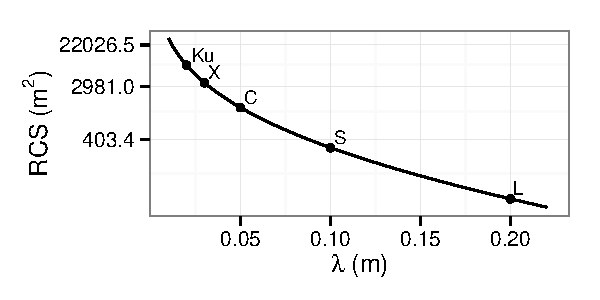
\includegraphics[width=\maxwidth]{figure/unnamed-chunk-2} 

}



\end{knitrout}



}
}

\question{1.3}
{A mid-C band radar has the following:

%\begin{align*}
%P_{avg} & = 1 \text{ kW}\\
%G & = 30 \text{ dB}\\
%\tau_\text{dwell} & = 30 \text{ ms}\\
%T_s & = 580\text{K}\\
%L & = 6 \text{ dB}
%\end{align*}

Calculate the maximum range at which it can detect a target of $\sigma=-20 \text{dBm}^2$. Assume the SNR required for detection is 17 dB and $C_B=1$.
}
{

The solution for this problem is accomplished by solving the radar equation for the Range ($R$) and substituting the above radar parameters after they are converted into matching dB scales.

\begin{align*}
\text{SNR} & = \frac{P_{avg}G^2\lambda^2\sigma\tau_\text{dwell}}{(4\pi)^3R^4kT_sC_BL} \\
\therefore R & = \left[\frac{P_{avg}G^2\lambda^2\sigma\tau_\text{dwell}}{(4\pi)^3(\text{SNR})kT_sC_BL}\right]^{\frac{1}{4}} \\
\end{align*}

In keeping with the world of sonar and radar, most quantites are calculated in dB space.  I now convert the above equation to dB form and substitute all the nessessary quantities.

\begin{align*}
R & = \left[\frac{P_{avg}G^2\lambda^2\sigma\tau_\text{dwell}}{(4\pi)^3(\text{SNR})kT_sC_BL}\right]^{\frac{1}{4}} \\
10\log_{10}(R) & = 10\log_{10}\left(\left[\frac{P_{avg}G^2\lambda^2\sigma\tau_\text{dwell}}{(4\pi)^3(\text{SNR})kT_sC_BL}\right]^{\frac{1}{4}}\right)\\
& = \frac{1}{4}\cdot 10 \left[\log_{10}(P_{avg}) + 2\log_{10}(G) + 2\log_{10}(\lambda) + \log_{10}(\sigma) + \log_{10}(\tau_\text{dwell})\right.\\
& \ \ \ \ \ \left. - 3\log_{10}((4\pi)) - \log_{10}(\text{SNR}) - \log_{10}(kT_s) - \log_{10}(C_B) - \log_{10}(L)\right]\\
& = \frac{1}{4}\left[40 + 60 + (-13.01) + (-20) + (-15.2) - 33 - 17 - (-201) - 0 - 7\right]\\
& = \frac{1}{4}(195.79) = 48.9 \text{ dBm}
\end{align*}

The solution of 48.9 is in the units of dBm which correlates to 77,600 m.
}

\question{1.4}
{A pulsed mid-X band radar has a maximum unambiguous velocity interval $\Delta \nu_\mu=600$ m/s. (Assume $\tau << \tau_R$.)}
{

\question{a}{What is its maximum unambiguous range $R_u$?}{
The first operation is to use the $\Delta \mu_\mu$ value stated to determine the $f_R$.  This can then be used to determine the maximum unambiguous range.  The value for $f_R$ is found in the following way:

\begin{align*}
\Delta \nu_\mu & = \frac{f_R \lambda}{2} \\
\therefore f_R & = \frac{2\Delta \nu_\mu}{\lambda} \\
& = \frac{(2)(600)(10\times 10^9)}{3\times 10^8} \simeq 4000 \text{ Hz}
\end{align*}

The maximum ambiguous range can then be found from the above value of $f_R$.

\begin{align*}
R_u & = \frac{c}{2f_R} \\
& = \frac{3\times 10^8}{(2)(4000)} \simeq 37500 \text{ m}
\end{align*}

}

\question{b}{Suppose its frequency is changed to mid-Ku band and other parameters remain the same. Calculate $\Delta \nu_\mu$ and $R_u$.}{

Altering the frequency to the mid-Ku band does not alter the structure of the pulses and therefore the maximum ambigious range remains the same at 37,500 m.  The shift in wavelength however does alter the maximum unambigious velocity interval.

\begin{align*}
\Delta \nu_\mu & = \frac{f_R\lambda}{2} \\
& = \frac{4000}{2}\cdot\frac{3\times 10^8}{10\times 10^9} \simeq 60 \text{ m/s}
\end{align*}

}
}

\question{1.5}{Calculate range gate width $\Delta R$ in both meters and feet for $\tau=0.01, 0.1, 1, \text{and} 10 \text{ } \mu$sec. What is the appropriate relationship between $\tau$ (nsec) and $\Delta R$ (feet)?}
{

% There are approximatly 0.3048 meters per foot or 3.2808 feet per meter  

The range gate is provided with the equation:

\begin{equation*}
\Delta R = \frac{c\tau}{2}
\end{equation*}




Results would typically be given in meters but the units can be transformed to feet by using the scaling factor of 3.2808 feet/meter.  The range gate width is:

\begin{center}
\begin{tabular}{l|ll} \hline
$\tau$ ($\mu$ s) & $\Delta R$ (meters) & $\Delta R$ (feet) \\ \hline
0.01 & 1500 & 4921 \\
0.1 & 15000 & 49212 \\
1 & 150000 & 492120 \\
10 & 1500000 & 4921200 \\
\end{tabular}
\end{center}

The equation listed above can have explicit scaling factors inserted to accept nanoseconds and report in feet by applying the appropriate conversion ratio, $\rho$.  The ratio is determined below:

\begin{equation*}
\rho = \frac{1 \text{ (m)}}{1 \text{ (sec)}}\cdot\frac{3.2808 \text{ (feet)}}{1 \text{ (m)}}\cdot\frac{1 \text{ (sec)}}{1\times 10^9 \text{ (nsec)}} \simeq 3.28\times 10^{-9}
\end{equation*}

The modified equation taking this scaling factor into account is:

\begin{equation*}
\Delta R = \frac{c\tau}{2}\rho \rightarrow \frac{\left(3\times 10^8\right)\tau}{2}\left(3.28\times 10^{-9}\right) \simeq 0.046\tau \text{ (feet)}
\end{equation*}

With this relationship, for each nanosecond of time you add to the pulse length, there is a corresponding increase of 0.05 feet in the range gate width.

}

\question{1.6}{A lossless radar with gain $G$ and wavelength $\lambda$ is located at a height $H$ above an infinite, flat planar, perfectly conducting surface, with boresight directed perpendicular to the surface. Compute $\Gamma$.}
{

Since the reflector is infinite in size and perfectly conducting, this problem can be reduced to the situation of an emitter that is exactly $2H$ away.  The received power is then going to be determined by assuming spherical spreading from the emitter and the cross-section of the receiving antenna.  This is taken directly from Equation 1.20 in the text.  In this case, $L\rightarrow 0$ since it is a lossless antenna and $R\rightarrow 2H$.  The modified equation is:

\begin{equation*}
\Gamma = \frac{G^2\lambda^2\sigma}{(4\pi)^3(2H)^4}
\end{equation*}

}


\end{document}
